\documentclass[10pt,landscape,a4paper]{article}
\usepackage[utf8]{inputenc}
\usepackage[ngerman]{babel}
\usepackage[T1]{fontenc}
%\usepackage[LY1,T1]{fontenc}
%\usepackage{frutigernext}
%\usepackage[lf,minionint]{MinionPro}
\usepackage{tikz}
\usetikzlibrary{shapes,positioning,arrows,fit,calc,graphs,graphs.standard}
\usepackage[nosf]{kpfonts}
\usepackage[t1]{sourcesanspro}
\usepackage{multicol}
\usepackage{wrapfig}
\usepackage[top=0mm,bottom=1mm,left=0mm,right=1mm]{geometry}
\usepackage[framemethod=tikz]{mdframed}
\usepackage{microtype}
\usepackage{pdfpages}
\usepackage[linguistics]{forest}

\let\bar\overline

\definecolor{myblue}{cmyk}{1,.72,0,.38}

\def\firstcircle{(0,0) circle (1.5cm)}
\def\secondcircle{(0:2cm) circle (1.5cm)}

\colorlet{circle edge}{myblue}
\colorlet{circle area}{myblue!5}

\tikzset{filled/.style={fill=circle area, draw=circle edge, thick},
    outline/.style={draw=circle edge, thick}}
    
\pgfdeclarelayer{background}
\pgfsetlayers{background,main}

\everymath\expandafter{\the\everymath \color{myblue}}
\everydisplay\expandafter{\the\everydisplay \color{myblue}}

\renewcommand{\baselinestretch}{.8}
\pagestyle{empty}

\global\mdfdefinestyle{header}{%
linecolor=gray,linewidth=1pt,%
leftmargin=0mm,rightmargin=0mm,skipbelow=0mm,skipabove=0mm,
}

\newcommand{\header}{
\begin{mdframed}[style=header]
\scriptsize
\sffamily
Hilfszettel zur Klausur\\
von~Tim~S.,~Seite~\thepage~von~2
\end{mdframed}
}

\makeatletter % Author: https://tex.stackexchange.com/questions/218587/how-to-set-one-header-for-each-page-using-multicols
\renewcommand{\section}{\@startsection{section}{1}{0mm}%
                                {.2ex}%
                                {.2ex}%x
                                {\color{myblue}\sffamily\small\bfseries}}
\renewcommand{\subsection}{\@startsection{subsection}{1}{0mm}%
                                {.2ex}%
                                {.2ex}%x
                                {\sffamily\bfseries}}



\def\multi@column@out{%
   \ifnum\outputpenalty <-\@M
   \speci@ls \else
   \ifvoid\colbreak@box\else
     \mult@info\@ne{Re-adding forced
               break(s) for splitting}%
     \setbox\@cclv\vbox{%
        \unvbox\colbreak@box
        \penalty-\@Mv\unvbox\@cclv}%
   \fi
   \splittopskip\topskip
   \splitmaxdepth\maxdepth
   \dimen@\@colroom
   \divide\skip\footins\col@number
   \ifvoid\footins \else
      \leave@mult@footins
   \fi
   \let\ifshr@kingsaved\ifshr@king
   \ifvbox \@kludgeins
     \advance \dimen@ -\ht\@kludgeins
     \ifdim \wd\@kludgeins>\z@
        \shr@nkingtrue
     \fi
   \fi
   \process@cols\mult@gfirstbox{%
%%%%% START CHANGE
\ifnum\count@=\numexpr\mult@rightbox+2\relax
          \setbox\count@\vsplit\@cclv to \dimexpr \dimen@-1cm\relax
\setbox\count@\vbox to \dimen@{\vbox to 1cm{\header}\unvbox\count@\vss}%
\else
      \setbox\count@\vsplit\@cclv to \dimen@
\fi
%%%%% END CHANGE
            \set@keptmarks
            \setbox\count@
                 \vbox to\dimen@
                  {\unvbox\count@
                   \remove@discardable@items
                   \ifshr@nking\vfill\fi}%
           }%
   \setbox\mult@rightbox
       \vsplit\@cclv to\dimen@
   \set@keptmarks
   \setbox\mult@rightbox\vbox to\dimen@
          {\unvbox\mult@rightbox
           \remove@discardable@items
           \ifshr@nking\vfill\fi}%
   \let\ifshr@king\ifshr@kingsaved
   \ifvoid\@cclv \else
       \unvbox\@cclv
       \ifnum\outputpenalty=\@M
       \else
          \penalty\outputpenalty
       \fi
       \ifvoid\footins\else
         \PackageWarning{multicol}%
          {I moved some lines to
           the next page.\MessageBreak
           Footnotes on page
           \thepage\space might be wrong}%
       \fi
       \ifnum \c@tracingmulticols>\thr@@
                    \hrule\allowbreak \fi
   \fi
   \ifx\@empty\kept@firstmark
      \let\firstmark\kept@topmark
      \let\botmark\kept@topmark
   \else
      \let\firstmark\kept@firstmark
      \let\botmark\kept@botmark
   \fi
   \let\topmark\kept@topmark
   \mult@info\tw@
        {Use kept top mark:\MessageBreak
          \meaning\kept@topmark
         \MessageBreak
         Use kept first mark:\MessageBreak
          \meaning\kept@firstmark
        \MessageBreak
         Use kept bot mark:\MessageBreak
          \meaning\kept@botmark
        \MessageBreak
         Produce first mark:\MessageBreak
          \meaning\firstmark
        \MessageBreak
        Produce bot mark:\MessageBreak
          \meaning\botmark
         \@gobbletwo}%
   \setbox\@cclv\vbox{\unvbox\partial@page
                      \page@sofar}%
   \@makecol\@outputpage
     \global\let\kept@topmark\botmark
     \global\let\kept@firstmark\@empty
     \global\let\kept@botmark\@empty
     \mult@info\tw@
        {(Re)Init top mark:\MessageBreak
         \meaning\kept@topmark
         \@gobbletwo}%
   \global\@colroom\@colht
   \global \@mparbottom \z@
   \process@deferreds
   \@whilesw\if@fcolmade\fi{\@outputpage
      \global\@colroom\@colht
      \process@deferreds}%
   \mult@info\@ne
     {Colroom:\MessageBreak
      \the\@colht\space
              after float space removed
              = \the\@colroom \@gobble}%
    \set@mult@vsize \global
  \fi}

\makeatother
\setlength{\parindent}{0pt}

\begin{document}
\graphicspath{ {inhalt/pictures/} }
%\footnotesize
\small
\begin{multicols*}{6}
\section{Fundamental Concepts}
\scriptsize{Reference} {\tiny How does the mapping between form and meaning work? Does it work at all?}\\
\scriptsize{Compositionality} {\tiny How are
complex utterances built from
smaller units? Are they built
from smaller units at all?}\\
\scriptsize{Combinatorial structure} {\tiny a small number of meaningless building blocks (phonemes, parts of syllables) combined into an unlimited set of utterances (words and morphemes)}\\
\scriptsize{Compositional structure} {\tiny meaningful building blocks (words and morphemes) are combined into larger meaningful utterances (phrases and sentences)}
\section{Dependency Grammar}
{\tiny curved arrows from the head to the dependent}\\
\scriptsize{auxiliary verbs}\\
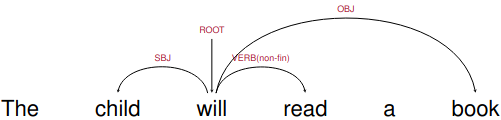
\includegraphics[scale=0.25]{auxiliary.png}\\
\scriptsize{Copular Clauses}\\
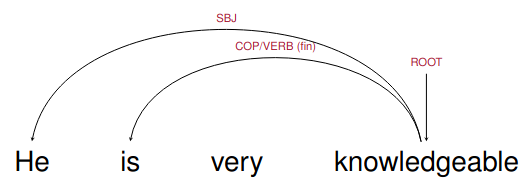
\includegraphics[scale=0.25]{copular.png}\\
\scriptsize{Dative Alternation}\\
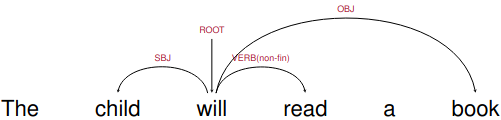
\includegraphics[scale=0.25]{auxiliary.png}\\
\scriptsize{Determiners} {\tiny DET, depends on the noun.}\\
\scriptsize{ADV} {\tiny depends on the verb or the ADV}\\
\scriptsize{ADJ} {\tiny depends on the noun}\\
\scriptsize{PP} {\tiny in PP, noun depends on preposition, other elements depend on the noun}\\
\scriptsize{POSS} {\tiny possessor depends on possessee}\\
\scriptsize{Complementizer Phrase} {\tiny complementizer (e.g. that) depends on the head-verb, itself is the head of the subordinate clause}\\
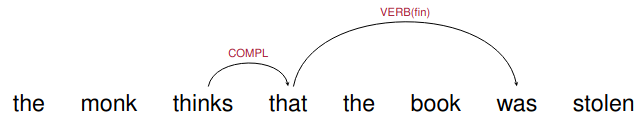
\includegraphics[scale=0.2]{complementizer.png}\\
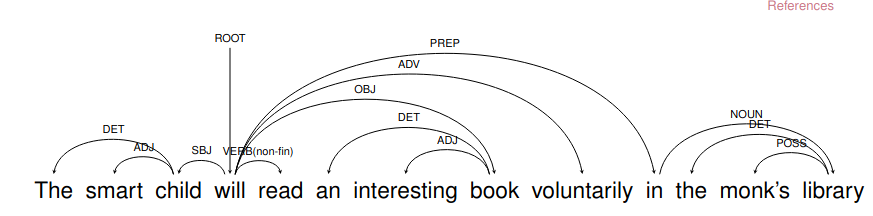
\includegraphics[scale=0.17]{DependencyGrammarExample.png}\\
\scriptsize{head-initial languages} {\tiny transitive sentences generally start with a verb, dependencies project forwards}\\
\scriptsize{head-final languages}
{\tiny dependencies project backwards}\\
\scriptsize{head-medial languages}
{\tiny dependencies project in both directions}\\
\scriptsize{linearization}
{\tiny dependency grammars often not not require particular rules
for the linearization of words; appropriate for languages with discontinuous constituents}\\
\scriptsize{free word order}
{\tiny linearization might not be required}\\
\scriptsize{fixed word order}
{\tiny lack of linearization constraints lincenses ungrammatical sentences}\\
\scriptsize{passive}\\
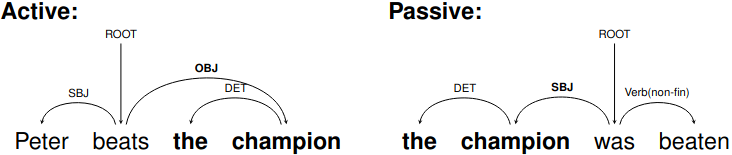
\includegraphics[scale=0.17]{passive.png}\\
\scriptsize{coordination}\\
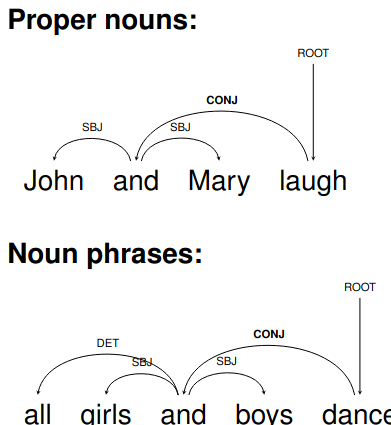
\includegraphics[scale=0.17]{coordination.png}\\
\scriptsize{crossing dependencies}
{\tiny non-projective}\\
\scriptsize{two competing pressures shpe word order}
{\tiny dependency length minimization; predictability maximization}
\section{Phrase Structure Grammar}
\scriptsize{Grammar g} {\tiny <T, NT, S, R>}\\
\scriptsize{Language} {\tiny set of all strings g can generate\\
L(PSG) = \{(the, child, reads, a, book), (a, child, reaeds, the, book), (the, book, reads, a, child), (a, book, reads, the, child)\}}\\
\scriptsize{Rewrite} {\tiny tree notation, rewrite notation and bracket notation are structurally equivalent}\\
\scriptsize{Feature of PSG} {\tiny strongly restrict the number of possible sentences via linearization constraints in the non-terminal rules}\\
\scriptsize{binarization constraint} {\tiny all rewrite rules have only 1 symbol on the left and maximally 2 symbols on the right}\\
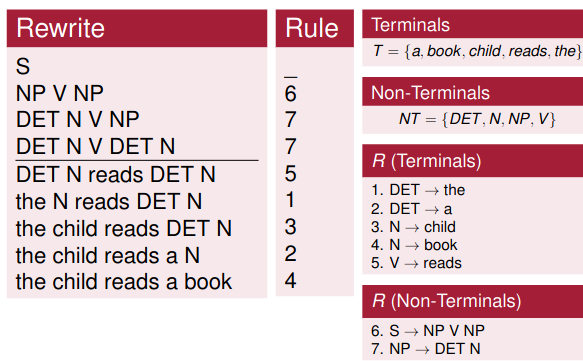
\includegraphics[scale=0.22]{psg.png}\\
\scriptsize{Expanding PSG}
{\tiny vocabulary, morphology}\\
\scriptsize{Problems}
{\tiny complicated agreement systems; implementing morphological features}\\
\scriptsize{verb position}
{\tiny verb-final, verb-medial, verb-initial, transitive, ditransitive (introduction of recursive rule will lead to generation of ungrammatical sentences}\\
\scriptsize{passive}
{\tiny VP -> AUX VP (aux: is), have to formulate different phrase structure rules for active and passive sentences}\\
\scriptsize{Pros}
{\tiny implements linearization constraints exlicitely; grounded on solid mathematical footing (automata theory); can be extended to model morphological features; easily implementable in computational frameworks}\\
\scriptsize{Cons}
{\tiny not all languages need rules (free word order); cumbersome to implement morphological features; excludes semantic aspects from grammaticality; infinite number of PSGs without further constraints}
\section{Chomsky Hierarchy}
\scriptsize{Notational Concentions}\\ {\tiny T: lower case Latin letters(e.g. a,b,c,x,y,z) \\
NT: upper case Latin letters(e.g. A,B,C,X,Y,Z) \\
strings of T and NT symbols: lower case greek letters(e.g. $\alpha, \beta, \gamma$ }\\
\scriptsize{Regular lanugages/finite state grammars/type 3}\\ {\tiny X -> x, 
X -> xY\\
(beware: different usages: X -> YZ where Y $\neq$ Z)\\
examples: set of strings following the pattern x**ny**m; set of strings such that number of 'a's is a multiple of 4; set of natural numbers that leave a remainder of 3 when divided by 5...\\
If...then...; either...or...; the..., is...; in natural languages cannot be generated by regular grammars\\
Limitations: for certain constructions, e.g. of the anbn typle, they will also generate ungrammatical sentences; since at least 1 terminal symbol has to be produced in every rewrite, no higher level patterns (phrase structures) can be captured
}\\
\scriptsize{Context-free languages/type 2}\\ 
{\tiny X -> $\beta$, only allow 1 single non-terminal on the left hand side, but an arbitrary string of terminals and non-terminals on the right hand side.\\
Examples of generated languages: \\
mirror langauge abba, abccba, acbddcba...\\
palidrome language: aba, bab, abba...\\
languages with form x**ny**mz**mw**n\\
Natural language not context-free? (Swiss German ambncmdn, Bambara)\\
Summary: more powerful than regular grammars; taken its binarized version, boils down to having 1 additional rule pattern compared to regular grammars X -> YZ (Y=Z allowed)
}\\
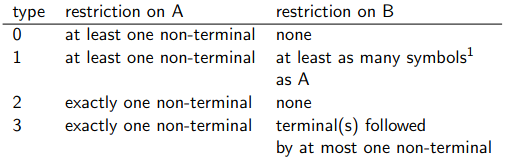
\includegraphics[scale=0.25]{chomsky.png}\\
\scriptsize{Context-sensitive languages/type 1}\\ {\tiny $\varphi_1 X \varphi_2 \to \varphi_1 \beta \varphi_2$, X is a single non-terminal X, the context may be null\\
alternative version: $\alpha \to \beta$, with $\beta$ at least as long as $\alpha$\\
example: copy language aa, abab, abcabc...\\
languages with strings of form x**ny**nz**n\\
set of all prime numbers (where each number represented by a string of length I(x))\\
assumption that natural languages are at least mildly context-sensitive
}\\
\scriptsize{Recursively enumerable languages/type 0}\\{\tiny $\alpha \to \beta$
}\\
\scriptsize{Classical hierarchy}\\ {\tiny regular (a**nb**m) finite-state automaton \\
context-free (a**nb**n) push-down automaton\\
context-sensitive (a**2**n) linear-bounded automaton\\
type-0 (a**n) Turing machine
}\\
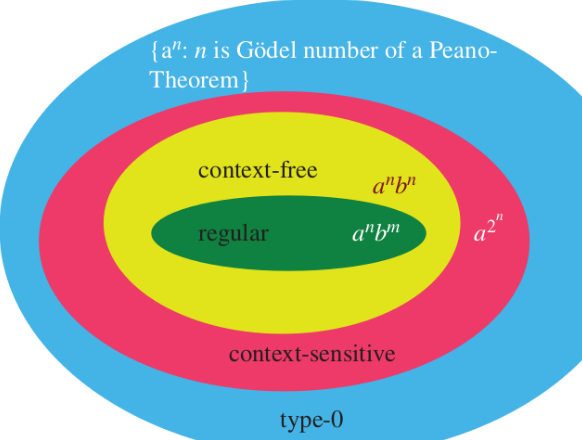
\includegraphics[scale=0.15]{chomsky-hierarchy.png}
\section{X-bar Theory}
{\tiny bars represent projection levels}\\
{\tiny introducing 2 bar-levels (e.g. NP and N-bar) allows us to apply recursiveness where necessary, but also avoid it where it would lead to ungrammatical structures}\\
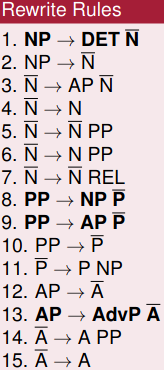
\includegraphics[scale=0.3]{xbar-rules.png}
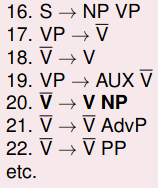
\includegraphics[scale=0.3]{xbar-rules2.png}\\
\scriptsize{X' rules} {\tiny the structural similarities be captured by use X as a placeholder, e.g. \\
X''->specifier'' X'\\
X'->adjunct''X', or X'->X' adjunct''\\
X'->X complement''}\\
\scriptsize{minimal and maximal X' phrases}\\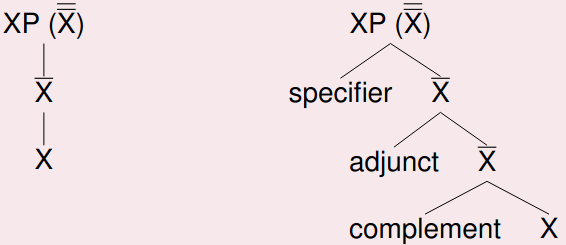
\includegraphics[scale=0.2]{xbar-min-max.png}\\
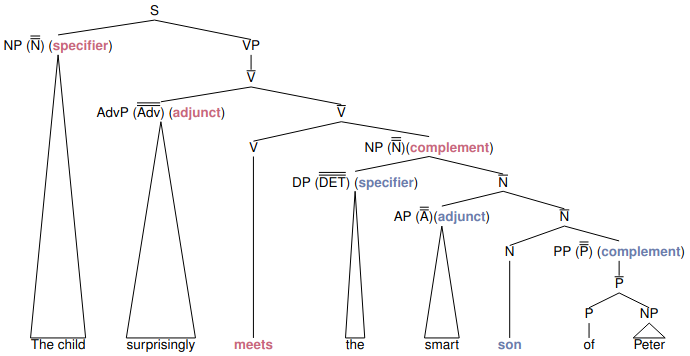
\includegraphics[scale=0.2]{xbar-max.png}\\
\scriptsize{Pros} 
{\tiny explicitely models the productiveness of natural language by recursively applying rules (but also possible in classical PSGs)\\
Abstracts away from particular phrase types and formulates more general rules (X-bar rules)\\
morphological features can be implemented}\\
\scriptsize{Cons} 
{\tiny an inflation of unary branches, analyses of simple sentences daunting\\
Justifying the higher level X rules based on empirical data (i.e. grammatical and ungrammatical sentences) becomes increasingly difficult and controversial.}
\section{Government \& Binding}
{\tiny Transformational Grammar and its subsequent incarnations (such as
Government and Binding Theory and Minimalism) were developed by
Noam Chomsky}\\
{\tiny The different implementations of Chomskyan theories are often grouped under the heading Generative Grammar, it comes from the fact that phrase structure grammars and the augmented frameworks that were suggested by Chomsky can generate sets of well-formed expressions }\\
\scriptsize{additional symbols:}\\ {\tiny C: Complementizer (subordinating conjunctions such as "that")\\
I: Finiteness (as well as Tense and Mood)\\
D: Determiner (article, demonstrative)
}\\
\scriptsize{projection levels} {\tiny X0: symbol that leads to the terminal symbol\\
X': intermediate projection \\
XP: highest projection (X'')
}\\
\scriptsize{Inflectional symbol INFL} {\tiny e.g. will, -s \\
both auxiliary and non-auxiliary constructions can be captured by the same underlying tree structure\\
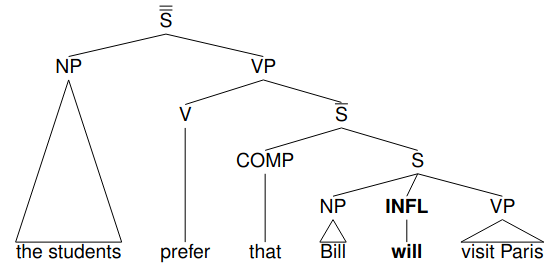
\includegraphics[scale=0.2]{infl.png}\\
problem: missing inflections, irregulars, language diversity\\
a structural analysis template that was developed for English}\\
\scriptsize{Deep Structure} {\tiny e.g. INFL VP}\\
\scriptsize{Surface Structure} 
{\tiny e.g. visit-s}\\
\scriptsize{CP and IP} 
{\tiny instead of S symbol, Complementizer Phrase and Inflectional Phrase as layers above the verb phrase\\
IP symbol essentially replaces the starting symbol S in GB analyses, the subject is considered the specifier of the IP, and the object is the complement of the IP\\
CP is yet another level above the VP, relevant when a complementizer is used, but also for other syntactic phenomena}\\
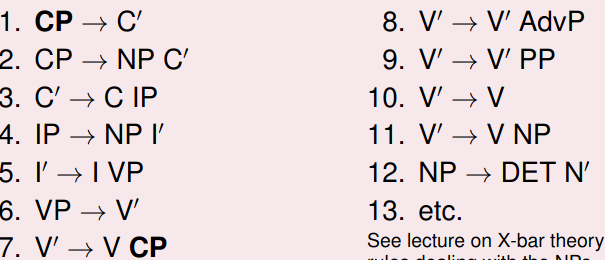
\includegraphics[scale=0.2]{cp-ip-rules.png}\\
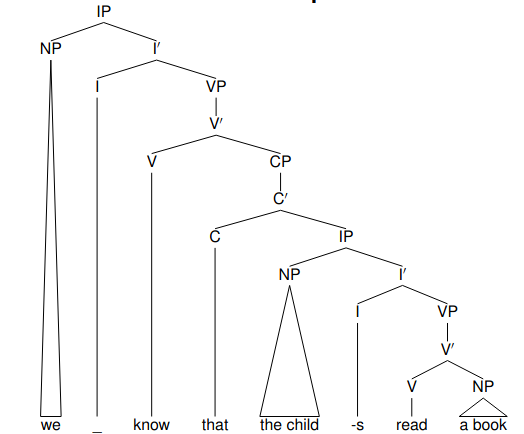
\includegraphics[scale=0.25]{GB_tree.png}\\
\scriptsize{Movement} 
{\tiny the verb moves up to the affix}\\
\scriptsize{Trace} 
{\tiny when an element moves into another position in the tree, it leaves a trace in the position where it was before}\\
\scriptsize{Pros} 
{\tiny Formulates a highly abstract and general template (D-Structure) which can be used to model all types of sentences and syntactic phenomena (at least aims to)}\\
\scriptsize{Cons} 
{\tiny requires many complicated mechanisms (movement, empty elements, case assignments...) to derive the set of possible sentences; lack of precise formulizations of these mechanisms has resulted in GB (and other Mainstream Generative Grammar approaches) being largely ignored by computational linguists}
\subsection*{Government}
{\tiny used in connection with case assignment between an I (e.g.will) and its specifier (e.g. the subject in nominative case), and between a verb head (e.g. read) and its complement (e.g. a book) in accusative/dative case)}\\
\scriptsize{case principle} {\tiny V assigns objective case (accusative) to its complements if it bears structural case\\
When finite, INFL assigns case to the subject\\
prepostions assign cases to the NPs they head\\
every maximum projection (XP) that dominates the NP that receives Case also dominates the head that assigns it
}\\
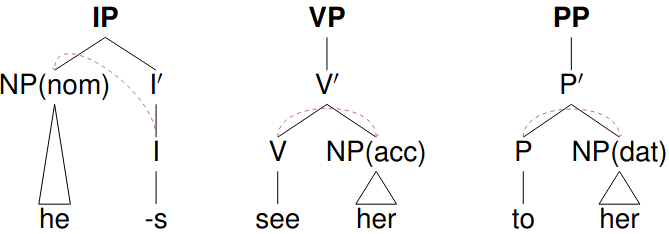
\includegraphics[scale=0.2]{case-assignment.png}\\
\scriptsize{Government} {\tiny alpha governs beta iff:\\
(i) alpha is a head, and \\
(ii) every XP that dominates alpha also dominates beta, and \\
(iii) every XP (other than IP) that dominates beta also dominates alpha\\
(dominate means a certain element is the mother-node or higher up in the tree of another element)
}\\
\scriptsize{problems} {\tiny unclear what exactly the relationship between case assignment and government is; case assignment can only work between some governor and a XP, unclear how this case then gets assigned to the elements further down the branches}
\subsection*{Binding}
{\tiny to determine when a reflexive anaphor, e.g. herself, is used instead of one of the pronouns she or her}\\
\scriptsize{Binding} {\tiny alpha binds beta iff:\\
(i) alpha does not dominate beta, \\
(ii) the mother-node that dominates alpha also dominates beta \\
(iii) alpha and beta are coindexed\\
(the first two clauses simply mean that alpha c-commands all categories below its own mother node)
}\\
\scriptsize{principles of binding theory} {\tiny (A) Pronouns (non-reflexive) must not be bound in their governing Inflectional Phrase (IP)\\
(B) reflexive Pronouns must be bound in their governing Inflectional Phrase (IP)\\
(C) Full NPs (aka denoting expressions) must not be bound\\
(accounts for the fact that the same full NP cannot be used again in ta single sentence, but have to be represented by a pronoun)\\
every maximum projection (XP) that dominates the NP that receives Case also dominates the head that assigns it
}\\
\scriptsize{problems} {\tiny several possible usages of reflexive and non-reflexive
pronouns do not conform to the rules of Binding Theory; no clear rules which NPs and pronouns are co-indexed.}
\subsection*{Syntactic Phenomena}
\scriptsize{T model} {\tiny (called by its shape when you invert it), a schematic representation of all the underlying processes assumed for generating well formed sentences in GB theory
}\\
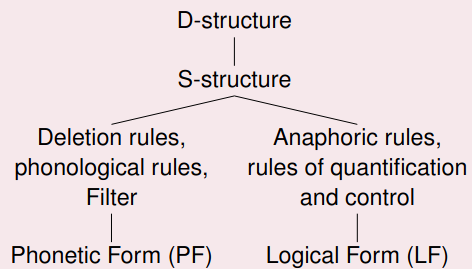
\includegraphics[scale=0.2]{t-model.png}\\
\scriptsize{D-Structure} {\tiny the underlying template or mould that is used to build all grammatical sentences in a given language}\\
\scriptsize{S-Structure} {\tiny derived by transformations which allow to move elements around and reassign cases\\
surface structure is not necessarily the actual string or phonemes that you might read or hear, deletions and phonetic rules might still apply}\\
\scriptsize{Deletion rules} {\tiny can be applied to the surface structure, indicated by underscores}\\
\scriptsize{Phonetic Form} {\tiny regular changes to the surface structure, e.g. wants to->wanna}\\
\scriptsize{Logical Form} {\tiny only marginally discussed, through binding theory (anaphora resolution)}\\
\scriptsize{Yes/No questions}\\
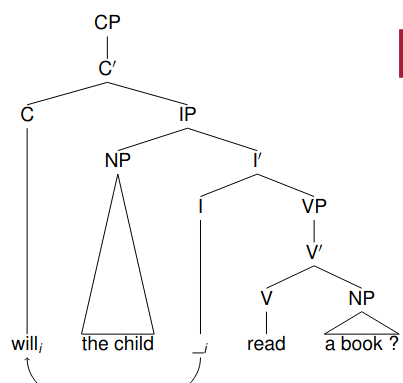
\includegraphics[scale=0.2]{yes-no.png}\\
\scriptsize{Wh-Questions}\\
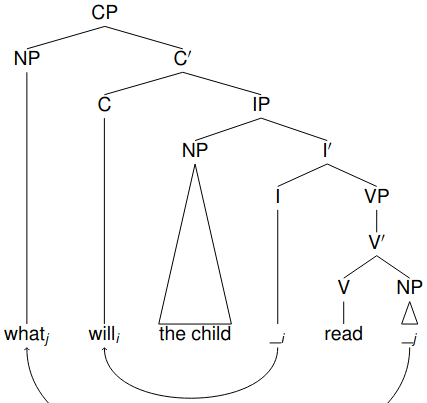
\includegraphics[scale=0.2]{what.png}\\
\scriptsize{Verb position} {\tiny verb position can be handled by flexibly changing the order of elements in the rewrite rules for IP and VP}\\
\scriptsize{parameters} {\tiny introduced to explain how variation (e.g. in verb position) across languages of the world can be explained against the backdrop of the same underlying deep structure}\\
\scriptsize{Fronting} {\tiny fronted element moved into positions of higher level phrases (CP and IP), like wh-movement or movement of auxiliaries in questions}\\
\scriptsize{Passive} {\tiny the same underlying deep structure as active constructions}\\
\scriptsize{Active(D-Structure)}\\
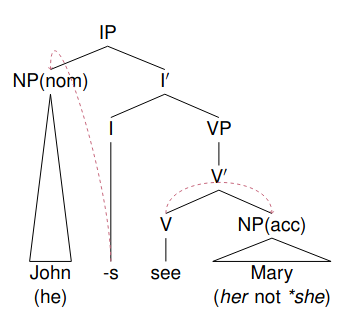
\includegraphics[scale=0.25]{GB_active.png}\\
\scriptsize{Passive(S-Structure)}\\
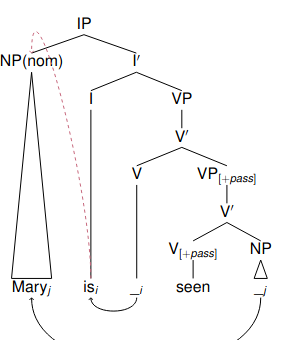
\includegraphics[scale=0.25]{GB_passive.png}\\
\scriptsize{Ditransitives} {\tiny problematic for GB analysis, need an additional recursive rule V'->V' NP\\
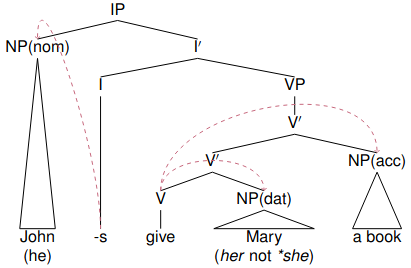
\includegraphics[scale=0.2]{ditransitive.png}\\
Problems: implies a verb can take arbitrarily large number of complements; run into problems with Binding Theory when reflexive pronouns are used}

\section{Minimalism}
\scriptsize{Features} {\tiny core part of minimalist syntax, refers to a feature value not a feature label, e.g. verbs might have the features past, plural, etc.
}\\
\scriptsize{categorial features} {\tiny POS, phrase symbol, e.g. A, N, V, NP, VP...
}\\
\scriptsize{$\phi$-features} {\tiny features relevant for agreement, e.g. PERSON, NUMBER, GENDER
}\\
\scriptsize{case features} {\tiny e.g. nominative, accusative}\\
\scriptsize{strong features} {\tiny features may be strong or weak, strong features make syntactic objects move to higher positions
}\\
\scriptsize{interpretable/uninterpretable features} 
{\tiny interpretable in English\\
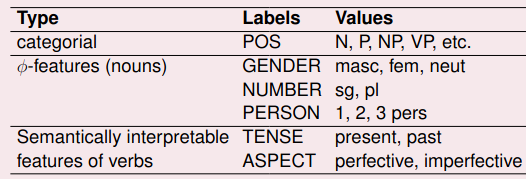
\includegraphics[scale=0.2]{interpretable.png}\\
uninterpretable in English\\
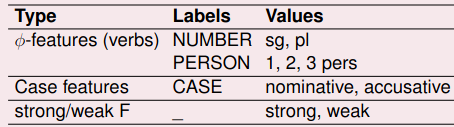
\includegraphics[scale=0.2]{uninterpretable.png}\\
differs corss-linguistically, e.g. GENDER feature is interpretable for English, not for German
}\\
\scriptsize{Feature Checking} 
{\tiny a core mechanism within Minimalist Syntax, links features with phrase structure, hence replaces traditional phrase structure rules\\
requirement: uninterpretable features must be checked, and once checked they delete\\
checking of categorial features: NP, NP with adjective, DP, VP\\
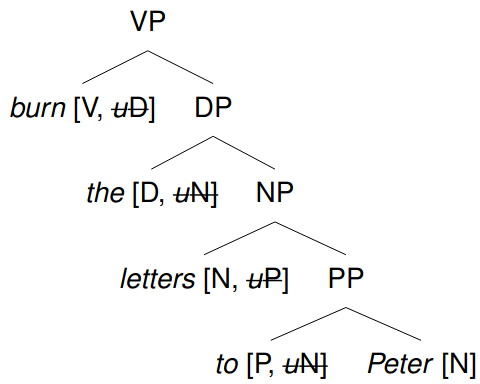
\includegraphics[scale=0.15]{feature-checking.png}\\
checking agreement features: Agree mechanism to check other features in addition to selectional features\\
agreement features can be checked in a sister node or further down the tree, whereas categorial features have to be checked in the sister node (or right below the sister node) of the feature to be checked\\
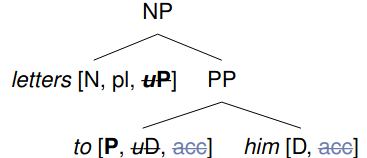
\includegraphics[scale=0.2]{agreement-features.png}
}\\
\scriptsize{Merge and Move} 
{\tiny
external merge (aka Merge): simply combines 2 elements like "the" and "book"\\
internal merge (aka Move($\alpha$): movement of constituents, adjoins some part of one linguistic object to the left of the respective object, the original position (i.e. trace) is indicated by <$\alpha$>\\
these have to be motivated by feature checking and essentially replaces phrase structure rules
}\\
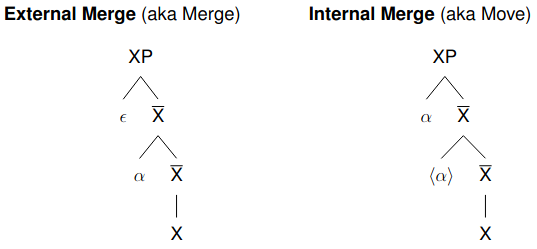
\includegraphics[scale=0.2]{merge.png}\\
\scriptsize{Phrase Structure} \\
{\tiny First merge - complements: combines a head with a single complement to create a complete phrase (XP)\\
Second merge - specifiers: combines a head with a specifier\\
little v: modelling ditransitives with reflexive pronouns, another higher level of the verb phrase, preferred by many practitioners of MP\\
Tense Phrase (TP): corresponds to IP in GB analysis\\
Complementizer Phrase (CP): in contrast to GB, full sentences in MP are always complementizer phrases; if C is empty, it still contributes to clause-type feature, e.g. Decl for declarative; the highest level phrase in MP\\
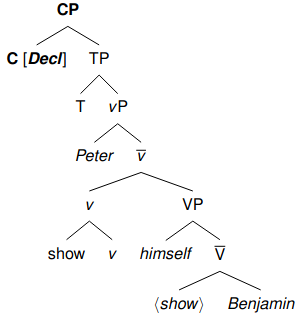
\includegraphics[scale=0.2]{cp.png}
}\\
\scriptsize{Differences between Minimalism and GB}
{\tiny structure building relies on feature checking not rewrite rules; there is just merge(external) and move(internal merge) applied in any order rather than D- and S- structure; case assignment no longer handled with the principle of government but by feature checking (Agree)}\\
\scriptsize{Pros}
{\tiny reduce the operations assumed for structure building (feature checking, merge and move) and hence more evolutionary plausible; 1 complement (first merge) and several specifiers (second merge) leads to a strictly binary structure without lots of unary branches (in X-bar theory)
}\\
\scriptsize{Cons}
{\tiny not fully formalized, hard to implement computationally; quickly fragmented into many divergent frameworks, development of implementations of large grammar fragments is hard
}
\section{Lexical Functional Grammar}
{\tiny developed in the 80s by Joan Bresnan and Ron Kaplan, they view LFG as a psycholinguistically plausible alternative to transformation-based approaches, forms part of West-Coast linguistics}\\
\scriptsize{Untyped Feature Descriptions} {\tiny matrices that contain inflectional\\
problem: syncretism, the same form fills different cells in inflectional paradigms -> use disjuction (or statement)\\
embedding: one feature description might be embedded in another feature description\\
path: a sequence of features which immediately follow each other, e.g. derivational morphology\\
list: we can use a list of feature values (and statment)\\
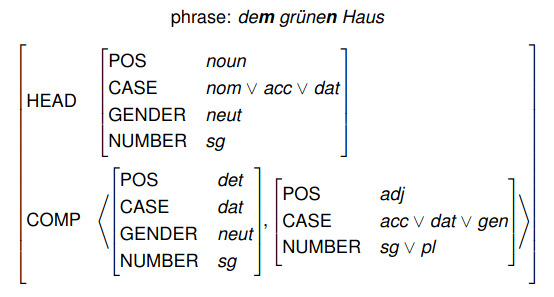
\includegraphics[scale=0.25]{untyped_feature_description.png}\\
}\\
\scriptsize{Typed Feature Descriptions} {\tiny i.e. feature structure, the type determines the template of feature labels that can be filled with values \\
inheritance: subordinate types inherit the features of their superordinate types\\
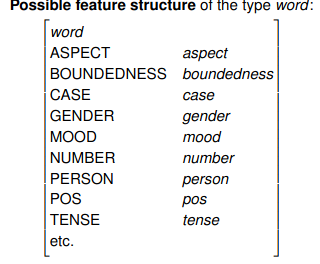
\includegraphics[scale=0.25]{type_word.png}\\
type hierarchies:\\
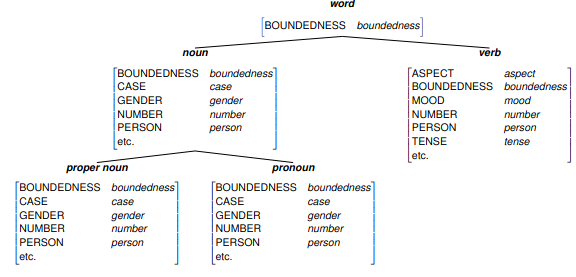
\includegraphics[scale=0.25]{type_hierarchy.png}
}\\
\scriptsize{Structure Sharing} {\tiny an identical feature structure is used in different parts of the feature description\\
e.g. agreement between determiner, adjective and noun in German:\\
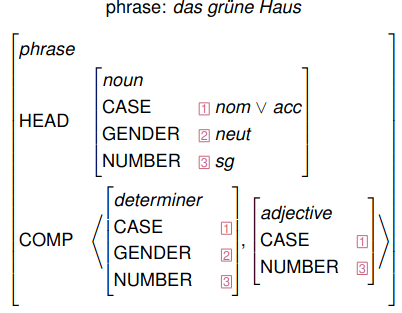
\includegraphics[scale=0.25]{agreement.png}\\
}
\scriptsize{Feature Descriptions and Structures}\\ 
{\tiny
A feature structure is a more general, stable model of all objects of a given type, while feature descriptions can give only (the relevant) parts of this model
}\\
\scriptsize{Grammatical Functions}\\ 
{\tiny e.g. PRED 'devour<SUBJ,OBJ>'}\\
\scriptsize{predicates (PRED)} 
{\tiny used for all lexical items that contribute meaning to the sentence, the value is either a lexical item(e.g.'David') or a lexical item followed by a list specifying grammatical functions (e.g.'devour<SUBJ,OBJ>')
}\\
{\scriptsize Syntactic Structure:\\
Argument Structure(A-Structure)
}\\
{\tiny general representation format: verb<x,y,z,ect.>\\
ordering: reflects a thematic hierarchy: agent>beneficiary>experiencer/goal>instrument>patient/theme>locative
}\\
\scriptsize{governable grammatical functions} 
{\tiny functions which have to be specidied by the head of the overall phrase/sentence\\
SUBJ, OBJ:object\\ $OBJ_{THEME}$:secondary object, direct object of a ditransitive sentence (e.g. gave \textit{the book}...)\\ COMP:sentential complement(that-clause)\\ OBL:oblique grammatical functions (e.g. $OBJ_{LOC}$: in..., at... after "located" (obligatory))
}\\
\scriptsize{non-governable grammatical functions} 
{\tiny functions that are not specidied by the head (not being arguments of the head)\\
ADJ(adjuncts), TOPIC, FOCUS(TOPIC and FOCUS can be used to model, e.g. word order variable when particular NPs are topicalized
}\\
\scriptsize{Functional Structure(F-Structure} 
{\tiny essentially a feature description for a whole phrase, e.g.:}\\
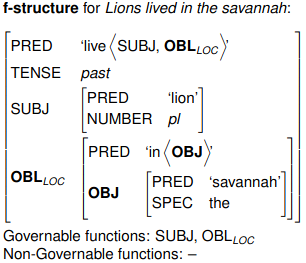
\includegraphics[scale=0.25]{f-structure1.png}\\
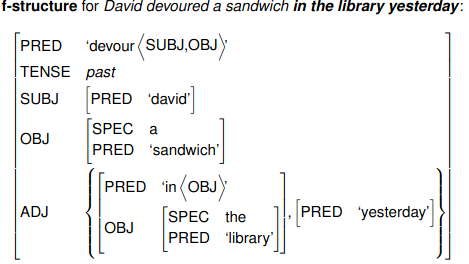
\includegraphics[scale=0.25]{f-structure3.png}\\
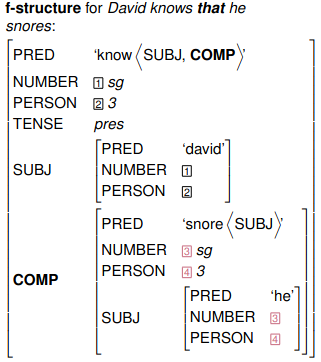
\includegraphics[scale=0.25]{f-structure2.png}\\
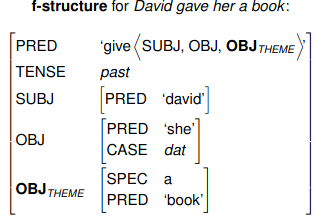
\includegraphics[scale=0.25]{f-structure4.png}\\
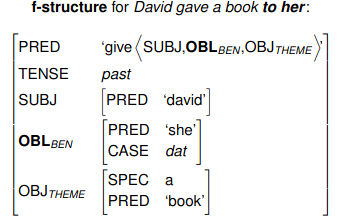
\includegraphics[scale=0.25]{f-structure5.png}\\
\scriptsize{Constituent Structure (C-Structure)} 
{\tiny licensed by (binary) phrase structure grammar, uses x-bar structures, e.g.:}\\
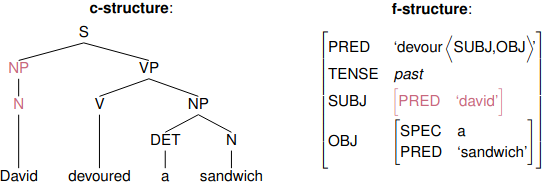
\includegraphics[scale=0.25]{c-structure1.png}\\
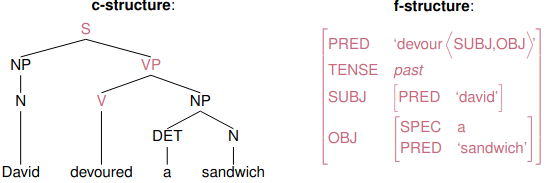
\includegraphics[scale=0.25]{c-structure2.png}\\
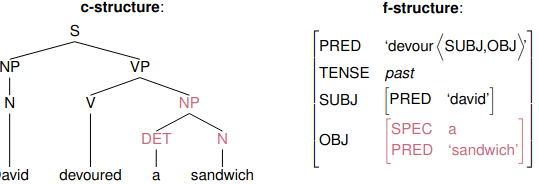
\includegraphics[scale=0.25]{c-structure3.png}\\
{\tiny summary: each structure models a different dimension of grammatical substance: role(a-structure), syntactic function(f-structure), phrase structure categories(c-structure)}\\
\scriptsize{Syntactic Phenomena\\
Passive} 
{\tiny simple mapping rule $verb<SBJ,OBJ> \to verb<(OBJ_{AG}),SBJ>$\\
translated into differing f-structures, valid for both configurational and non-configurational languages
}\\
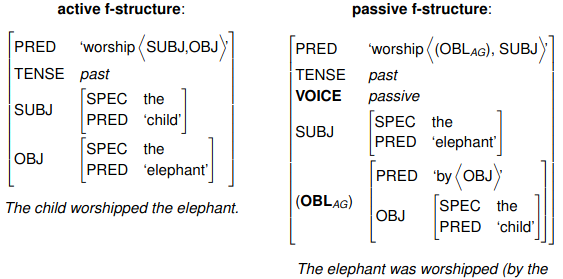
\includegraphics[scale=0.25]{LFG_passive.png}\\
\scriptsize{Pros} 
{\tiny fully formalized, computationally implementable\\
flexibility to deal with configurational(fixed word order) and non-configurational(flexible word order) languages\\
agreement and case assignment are modelled explicitely in the feature descriptions(similar to GPSG)\\
feature descriptions allow for analyses of long-distance dependencies and passive constructions without recurrence to transformations
}\\
\scriptsize{Cons} 
{\tiny Feature descriptions are untyped, which means that generalizations in terms of type hiearchies such as inheritance of features are not available (in contrast to HPSG)\\
the interactions between a-structure, f-structure, and c-structure are not straightforward, and will require a considerable amount of implementational details 
}
\section{Construction Grammar}
{\tiny like LFG and HPSG, Construction Grammar forms part of West Coast linguistics. It has been considerably influenced by Charles Fillmore, Paul Key and George Lakoff and Adele Goldberg}\\
\scriptsize{Goldbergian Construction Grammar}\\
\scriptsize{Construction} {\tiny Any linguistic pattern is recognized as a construction as long as some aspect of its form or function is not strictly predictable from its component parts or from other constructions recognized to exist\\
patterns are stored as constructions even if they are fully predictable as long as they occur with sufficient frequency, e.g. What be[fin] X doing Y?\\
all levels of grammatical analysis involve constructions: morpheme, word, complex word, idiom, covariational conditional, ditransitive, passive
}\\
\scriptsize{Notational Confusion} {\tiny for consistency, we use POS symbols, if necessary, can be further specified by indices\\
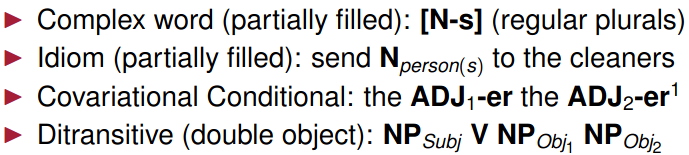
\includegraphics[scale=0.15]{CxG_notation.png}
}\\
\scriptsize{Multiple Constructions} {\tiny
an actual expression typically involves the combination of different constructions\\
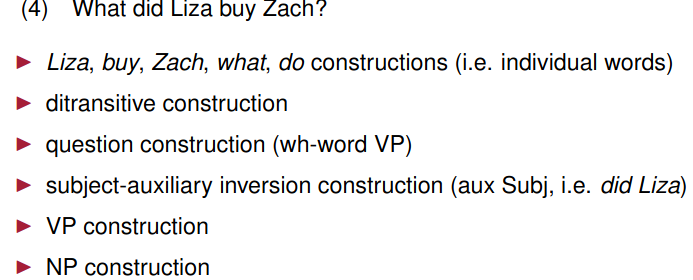
\includegraphics[scale=0.15]{multiple_construc.png}
}\\
\scriptsize{Arguments for Constructions}\\ {\tiny 1. creativity/productivity: the idea that main verbs specify the valency of whole sentences does not match the creative use of linguistic patterns\\
2. non-compositionality: many examples across languages where the overall meaning of a sentence is not derivable from the component parts but is rather assigned to the whole construction\\
3. core and periphery: constructions, while often seen to be part of the periphery, might in fact constitute a core property of language
}\\
\scriptsize{Pros}\\ 
{\tiny not based on an arbitrary distinction between core and periphery of grammar, but tries to cover all linguistic strcutures within the same framework\\
has (arguably) high psycholinguistic relevance for both learning and processing\\
abandons the ideas of headedness and valency, more flexible to deal with the productivity and creativity of languages
}\\
\scriptsize{Cons}\\ 
{\tiny unclear how to identify constructions without recurrence to more traditional analyses such as phrase structure rules and constituency\\
often only partially formalized, Müller argues that all fully formalized CxG variants are virtually equivalent to HPSG(since they largely use the same formal apparatus} 
\section{Semantics}
\scriptsize{Form and meaning: The Roots} \\
{\tiny Level 1: Abstract Relation\\
Level 2: Concrete Mapping (Denotation)\\
Level 3: Metalanguage (Translation)
}\\
\scriptsize{Arbitrariness} {\tiny For most words, the relation between the form (i.e. phonetic shape) of the word and its meaning is arbitrary; Onomatopoetic words are words whose forms are intended to be imitations of the sounds which they refer to. systematic non-arbitrariness, iconicity, systematicity}\\
\scriptsize{Compositionality} {\tiny two words might be productively combined to yield a new, predictable meaning. Hallmark of human language (and other communication systems) as it enables the infinite use of finite means. In the case of idioms (e.g. kicking the bucket), the intended meaning of the sentence is not a linear combinatorial derivation of its parts. Rather, a complex meaning is assigned to the whole phrase.}\\
\scriptsize{3 levels of meaning} {\tiny word meaning: sentence meaning, utterance meaning}\\
\scriptsize{Reference} {\tiny intuitively we are talking about the speaker’s use of words to “point to” something in the world}\\
\scriptsize{Semiotic Triangle(Triangle of Reference/Meaning)} {\tiny Symbol(language) - World(referent) - Thought/Reference(meaning)}\\
\scriptsize{Denotational Semantics} {\tiny focuses on the link between linguistic expressions and the world}\\
\scriptsize{Cognitive Semantics} {\tiny focuses on the link between linguistic expressions and mental representations}\\
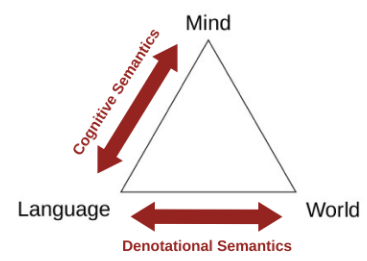
\includegraphics[scale=0.15]{triangle.png}\\
\scriptsize{Referring Expressions}\\ {\tiny Proper names (Mao Zedong)/rigid designators\\
“Natural kind” terms (the octopus, humans, methane): names of species or substances\\
Deictic elements (indexicals: you, here, now): words which refer to something in the speech situation itself.\\
Anaphoric elements (George... he..., every boy(non-referring anaphora))\\
Definite descriptions (this book, the sixteenth president): normally used in contexts where the hearer is able to identify a unique referent, but can also be used generically without referring to any specific individual \\
Indefinite descriptions (a cowboy): may be used to refer to a specific individual or may be non-specific, referring/non-referring/ambiguous
}\\
\scriptsize{Sense/Denotation}\\ {\tiny Sense: the aspects of meaning which do not depend on the context of use\\
Denotation: the sort of meaning which does depend on the context
}\\
\scriptsize{Word meaning}\\ {\tiny problem of variable reference, i.e. ambiguity, indeterminacy, vagueness\\
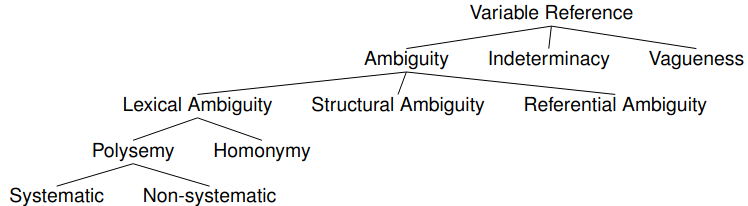
\includegraphics[scale=0.15]{variable-reference.png}\\
lexical ambiguity [ambiguous, polysemous] (e.g. beat): words that have two or more senses\\
structural ambiguity (e.g. Two cars were reported stolen by the Groveton police yesterday): the two senses arise because the grammar of the language can assign two different structures to the same string of words, even though none of those words is itself ambiguous\\
referential ambiguity: usage of anaphoric expressions with ambiguous antecendents
}\\
\scriptsize{Lexical Ambiguity}\\ {\tiny polysemy: one word with multiple senses (e.g. beat) (criteria: semantic feature/component sharing, figurative extension, existence of a primary sense, etymology)\\
homonymy: different words that happen to sound the same (e.g. can)\\
another perspective: allows for greater ease of processing by permitting efficient linguistic units to be re-used; a functional property of language that allows for greater communicative efficiency
}\\
\scriptsize{Indeterminacy} {\tiny a word can have variability in its reference despite having a single defined sense (e.g. cousin) 
}\\
\scriptsize{Vagueness} {\tiny limits of its possible denotations cannot be precisely defined (e.g. tall)
}\\
\scriptsize{Indeterminacy vs. Vagueness}\\ {\tiny context-dependence: denotation of a vague word depends on the context\\
borderline cases: vague words display borderline cases due to their gradability\\
"little-by-little" paradoxes: due to the gradability of vague words, it is hard (impossible?) to determine when a certain denotation is justified (e.g. when exactly does a person with hair become a bald person?)\\
indeterminacy tends to be language-specific, the degree to which these properties are preserved in translation
}\\
\scriptsize{Tests}\\ {\tiny Zeugma Test: on his fishing trip he caught three trout and a cold (lexically ambiguous)\\
Identity Test: John saw her duck, and so did Bill (lexically ambiguous: interpretations have to be identical)\\
Sense Relations Test: light - dark, heavy (different sets of synonyms, antonyms)\\
Contradiction Test: They are not children any more, but they are still my children (true, ambiguous)
}
\subsection*{Propositional Logic}
Why formal logic? {\tiny overcome ambiguity, determine relationships between meanings of sentences, determine meanings of setences, model compositionality, recursive system.}\\
\textbf{Definition}
Proposition {\tiny The meaning of a simple declarative sentence. The proposition expressed by a sentence is the set of possible cases [situations] of which that sentence is true.} \\
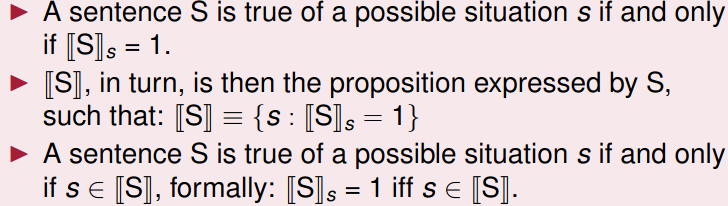
\includegraphics[scale=0.15]{proposition.png}\\
Extensions {\tiny real-world situations they refer to} \\
Frege’s Generalization {\tiny The extension of a sentence S is its truth value} \\
Types of Sentences and Propositions {\tiny Analytic sentence(tautology): true in every situation; Contradiction: false in every situation; Synthetic sentence: either true or false depending on the situation}\\
Inference {\tiny premisses: the facts which form the basis of the inference; conclusions: the fact which is inferred}\\
Syllogism {\tiny an important variety of deductive argument in which a conclusion follows from two or more premises}\\
Categorical Syllogism {\tiny A logical argument consisting of exactly three categorical propositions, two premises and the conclusion}\\
Types of Inference {\tiny inferences based on content words; logical words(propositional logic); quantifiers(predicate logic)}
\subsection*{Predicate Logic}
{\tiny Introduce constants and variables representing invididuals and predicates to capture the main structural building blocks of sentences. Introduce quantifiers to allow for quantified statements.}
\textbf{Definition}
{\tiny constant symbols: a, b, c\\
variable symbols: x, y, z\\
n-ary/n-place predicate symbols: A, B, C, reflect relations between n elements (n>0)\\
function symbols: lower case letters (f, g, etc.), take n variables (with n>=0) as their arguments, e.g. f(x): father of x\\
connectives:$\neg, \land, \lor, \to, ...$ \\
quantifiers: $\forall, \exists$ \\
round brackets (), equal sign =}\\
Universal instantiation {\tiny By using a variable x bound by the universal quantifier (Premise 1), and then specifiyng this variable as a constant symbol (Premise 2)}\\
Existential Generalization {\tiny By asserting that two predicates are true for the same constant symbol (premise 1 and premise 2)}\\
Evaluation: Model theory {\tiny a model: (i) the domain, i.e. the set of all individual entities in the situation, (ii) the denotation sets for the basic vocabulary items\\
N-place predicates are evaluated by whether the constant symbol(s) is a member of the denotation set of the predicate\\
Logical operators are evaluated the same way as in propositional logic\\
Quantifiers are evaluated according to subset relations
}\\
Valency in Semantics\\
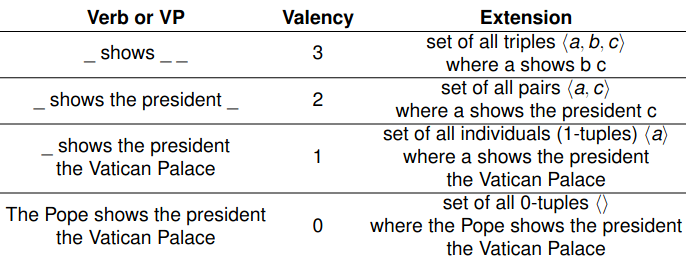
\includegraphics[scale=0.15]{valency.png}\\
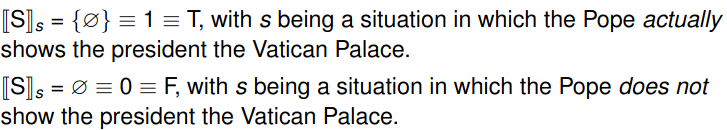
\includegraphics[scale=0.15]{0-valence.png}\\
Formal Composition {\tiny Compositional semantic theories assume that syntax and semantics work in parallel. For each phrase structure rule that combines two expressions into a larger phrase, there is a corresponding semantic rule which combines the meanings of the parts into the meaning of the newly formed expression}\\
Type theory {\tiny a formal semantic account enabling compositionality from the most basic entities (type e) to sentences (type t) in a recursive manner\\
Syntactic trees (here PSG trees) can then be mapped onto type-theoretic trees
}\\
Functional Application {\tiny If $\alpha$ is of type <b, a> and $\beta$ of type b, then $\alpha(\beta)$ is of type a}\\
\includegraphics[scale=0.15]{types.png}\\

%\section{Evidentiality}
covers the way in which information was acquired, without necessarily relating to the degree of speaker’s certainty concerning the statement or whether it is true or not. To be considered as an evidential, a morpheme has to have ‘source of information’ as its core meaning; that is, the unmarked, or default
interpretation.
\subsection*{Definition}
\emph{1st claim}: It is a “linguistic category”, i.e. a grammatical category with grammatical markers (same as for modality).\\
\emph{2nd claim}: These evidential markers have source of information as their core meaning.\\
markers can develop polysemy, e.g. tense marking and evidential marking, can be used recursively without being redundant\\
\emph{3rd claim}: Evidentiality is not “necessarily relating to the degree of speaker’s certainty”, i.e. it is distinct from epistemic modality.
\subsection*{Evidentiality vs. Epistemic Modality}
There is good evidence that evidential markers in a number of languages do not contribute to propositional content but function as illocutionary modifiers, and so must be distinct from epistemic modality.\\
\emph{Negation Test}: If negation can scope over the evidential marker, then the evidential marker is considered to contribute to the truth-conditional content.\\
\emph{Challenge Test}: The hearer can challenge the truth of the statement of the
speaker given more direct evidence, but the source of information cannot be challenged.\\
Two types of evidentials:\\
\emph{Illocutionary}: markers of evidentiality that do not contribute to the truth-conditional content, but that “add to or modify the sincerity conditions of the [speech] act”\\
\emph{Propositional}: markers of evidentiality that also contribute to the truth-conditional content. e.g. Es soll regnen.
\subsection{Cross-Linguistic Variation}
Semantic distinctions of evidentiality: no grammatical evidentials/indirect only/direct and indirect\\
Coding of Evidentiality: no grammatical evidentials/verbal affix or clitic/part of the tense system/separate particle/modal morpheme/mixed
%\section{Introduction to Pragmatics}
Semantics: word meaning, sentence meaning
Pragmatics: utterance meaning
\subsection*{Definitions}
\emph{Anomaly Definition}:study of those principles that will account for why a certain set of sentences are anomalous, or not possible
utterances.\\
\emph{Functional}: attempts to explain facets of linguistic structure by reference to non-linguistic pressures and causes.\\
\emph{Context}: part of performance, explicate the reasoning of speakers and hearers in working out the correlation in a context of a sentence token with a proposition.\\
\emph{Grammaticalization}: study of those relations between language and context that are grammaticalized, or encoded in the structure of a language.\\
\emph{Truth-Conditional}: those aspects of the meaning of utterances which cannot be accounted for by straightforward reference to the truth conditions of the sentences uttered.\\
\emph{Inter-Relation}: interation of context-dependent aspects of language structure and principles of language usage, relations between
language and context\\
\emph{Appropriateness/Felicity}: study of the ability of language users to
pair sentences with the contexts in which they would be
appropriate.\\
\emph{List}: study of deixis (at least in part), implicature, presupposition, speech acts, and aspects of
discourse structure.\\
More promising: Inter-Relation, Truth-Conditional
%\section{Discourse Representation Theory}
To deal with issues in the semantics and pragmatics of anaphora and tense\\
Discourse representation structures:a hearer builds up a mental representation of the discourse as it unfolds, and that every incoming sentence prompts additions to that representation. 
\subsection*{Anaphora Resolution}
Anaphora as co-reference: \emph{John} likes \emph{his} donkey.\\
Anaphora as binding: \emph{No farmer} likes \emph{his} donkey.\\
Anaphora as neither co-reference nor binding: John owns \emph{a donkey}. \emph{It} is grey.\\
\subsection*{Discourse Representation Structures}
Merging: [x, y: farmer(x), donkey(y), chased(x,y)] + [v, w: caught(v, w)] = [x, y, v, w: farmer(x), donkey(y), chased(x,y), caught(v, w)]\\
Anaphora Resolution: = [x, y, v, w: v=x, w=y, farmer(x), donkey(y), chased(x,y), caught(v,w)] = [x, y: farmer(x), donkey(y), chased(x,y), caught(x,y)]
\subsection*{Complex DRS Conditions}
\emph{Negation}: John doesn't own a donkey. It is grey. [1x,z: John(x), $\neg$[2y: donkey(y), owns(x,y)], grey(z)]. y is not accessible to z. x and z are accessible to y.\\
\emph{Conditionals}: If John owns a donkey, he likes it. [1:[2x,y: John(x), donkey(y), owns(x,y)]$\to$[3v,w: likes(v,w)]]=[1:[2x,y,v,w: v=x, w=y, John(x), donkey(y), owns(x,y)]$\to$[3: likes(v,w)]]=[1:[2x,y: John(x), donkey(y), owns(x,y)]$\to$[3: likes(x,y)]]. x and y are accessible to v and w.\\
\emph{Quantification}: Every farmer who owns a donkey, likes it. [1:[2x,y: farmer(x), donkey(y), owns(x,y)]$\forall x$[3v,w: likes(v,w)]]
%\section{Implicature}
Tools to get to grips with frequent compositional structures in natural language (adj-n, adv-v, art-n, prep-np... combis), a higher-order logic
\subsection*{Grice's Maxims}
\emph{The cooperative principle}: contribution as required\\
\emph{Maxim of Quality}: nothing false or lacks evidence\\
\emph{Quantity}: as informative as required\\
Relation(or Relevance)\\
\emph{Manner}: clear and easy to understand\\
Failure to fulfill a maxim:\\
(i) quietly violate a maxim. Politician: Yes, this is what we stand for.\\
(ii) opt out from adhering to the maxim or the cooperative principle. Politician: I won’t answer this question.\\
(iii) a clash, impossible to adhere to one maxim without not adhering to another. Politician: We are still deciding on the matter. I’m hopeful that
yes, but I cannot tell you for sure.\\
(iv) flout a maxim. Politician: I personally think this is a good idea.
\subsection*{Conversational Implicature}
a type of pragmatic inference about what is said by the speaker (literal meaning) in relation to what they actually intend to convey (communicative intention).\\
\emph{Group A}: no maxim is violated. {\tiny A: C doesn’t seem to have a partner these days. B: He/she has been paying a lot of visits to New York lately. Implicature: He/she might have a partner in New York.}\\
\emph{Group B}: a maxim is violated, can be explained by a clash with another maxim. {\tiny A: Where does C live? B: Somewhere in the South of France. Implicature: I don’t know the exact name of the place where C lives.}\\
\emph{Group C}: exploitation, a maxim is flouted for the purpose of deliberately creating a conversational implicature. {\tiny Recommendation letter: Dear B, C’s command of English is excellent, and he has attended tutorials regularly. Kind regards, A. Implicature: I cannot recommend C as a philosopher.}\\
\subsection*{Types of Implicature}
Conversational Implicatures:\\
\emph{Particularized}: the intended inference depends on particular features of the specific context of the utterance. {\tiny A: C managed to brake his car and get arrested for arrousing
public annoyance when he was drunk last night.
B: Yeah, he is smart like that.}\\
\emph{Generalized: Scalar, Connectives, Indefinite}: does not depend
on specific features of the utterance
context, but is instead normally implied by
any use of the triggering expression in
ordinary contexts.\\
\emph{Scalar}: non-maximal degree modifiers. {\tiny The water is warm -> The water is not hot. John has most of the documents -> John does not have all of the documents}\\
\emph{Connectives}: sentence connectives. {\tiny Susan gave Peter the key and Peter opened the door. -> She gave him the key and then he opened the door. Peter is either Susan’s brother or her boyfriend -> The speaker does not know whether Peter is Susan’s brother or boyfriend.}\\
\emph{Indefinites}: indefinite article. {\tiny I walked into a house. -> The house was not my house.}\\
Conventional Implicatures: \\
not context-dependent or pragmatically explainable [in contrast to conversational implicatures], and must be learned on a word-by-word basis. (controversial, similar to presuppositions?){\tiny Alfred has still not come -> His arrival is expected. I was in Paris last spring too -> Some other person was in Paris last spring. Even Bart has passed the test -> Bart was among the least likely to pass the test}
\subsection*{Entailment}
1. whenever p is true, it is logically necessary that q is also true;\\
2. whenever q is false, it is logically necessary that p is also false;\\
3. these relations follow from the meanings of p and q, independent of the context of utterance\\
{\tiny I broke your Ming dynasty jar (lexical) -> Your Ming dynasty jar is broken. Hong Kong is warmer than Beijing (comparative) -> Beijing is cooler than HK}\\
\subsection*{Tests}
\begin{tabular}{c c c c}
 &Entailment&Convers. Implicature&\\
cancellable&no&yes&\\
suspendable&no&yes&\\
reinforceable&no&yes&\\
negation&no&no&\\
question&no&no&\\
\end{tabular}
\emph{Cancellation} {\tiny HK is warmer than BJ, but BJ is not cooler than HK (NO). There is a garage around the corner, but unfortunately you cannot buy petrol there (YES)}\\
\emph{Suspension} {\tiny HK is warmer than BJ, but I'm not sure if BJ is cooler than HK (NO). There is a garage around the corner, but I'm not sure if you cannot buy petrol there (YES)}\\
\emph{Reinforcement} {\tiny HK is warmer than BJ, and BJ is cooler than HK (NO). There is a garage around the corner, and you cannot buy petrol there (YES)}\\
\emph{Negation} {\tiny HK is not warmer than BJ (BJ is cooler than HK: NO). There is no garage around the corner (you cannot buy petrol there: NO)}\\
\emph{Question} {\tiny Is HK warmer than BJ? (BJ is cooler than HK: NO). Is there a garage around the corner? (you cannot buy petrol there: YES)}\\
%\section{Presupposition}
information which is linguistically encoded as being part of the common ground at the time of utterance. {\tiny common ground: everything that both the speaker and hearer know or believe, and know that they have in common.}\\
Statement A and presupposition B: (i) if A is true, then B is true (ii) if A is false, then B is still true.\\
\subsection*{Presupposition Triggers}
\emph{Definite descriptions}: definite noun phrases, possessive phrases, restrictive relative clauses. e.g. the, my, the man who can fly\\
\emph{Factive predicates}: regret, be aware, realize, be sorry, know\\
\emph{Implicative Predicates}: manage to, forget to (presupposes other predicates, e.g. try to, intend to, to be true)\\
\emph{Aspectual Predicates}: express the beginning, stopping, continuing of events. e.g. stopped, has begun, continues to, resume\\
\emph{Temporal clauses}: before, after, by the time, while\\
\emph{Counterfactuals}: If I were..., If you had not...I would not have...\\
\emph{Comparisons}: as unreliable as, as old as...\\
\emph{Scalars}: more, some...\\
\subsection*{Accomodation and Failure}
\emph{Accomodation}: hearers accept the presupposition as true, or they might ask for confirmation to “officially” establish the presupposition as common ground\\
\emph{Failure}: the hearer rejects the presupposition\\
\emph{Group C}: exploitation, a maxim is flouted for the purpose of deliberately creating a conversational implicature. {\tiny Recommendation letter: Dear B, C’s command of English is excellent, and he has attended tutorials regularly. Kind regards, A. Implicature: I cannot recommend C as a philosopher.}\\
%\section{Speech Acts}
information which is linguistically encoded as being part of the common ground at the time of utterance. {\tiny common ground: everything that both the speaker and hearer know or believe, and know that they have in common.}\\
Statement A and presupposition B: (i) if A is true, then B is true (ii) if A is false, then B is still true.
\subsection*{Performatives}
indicative mood and present tense, use of performative verb(e.g. sentence, declare, confer, invite, request, order, accuese...), active void of a first person subject, usage of performative adverb ´hereby’.\\
\emph{Felicity Conditions}:\\
A.1 Conventionality Condition\\
{\tiny accepted conventional procedure}\\
A.2 Appropriateness Cond.\\
{\tiny appropriate persons and circumstances}\\
B.1 Correctness Cond.\\
B.2 Completeness Cond.\\
{\tiny procedure executed correctly and completely}\\
C.1 Sincerity Cond.\\
{\tiny person must intend so}\\
C.2 Subsequent Conduct Cond.\\
{\tiny person must subsequently conduct so}\\
\emph{Violations of Conditions}:\\
Misfire: conditions under A-B violated\\
Abuse: conditions under C violated\\
All sentences can be paraphrased as performatives
\subsection*{Speech Acts}
\emph{Locutionary Art}: The act of performing an utterance (phonetically and grammatically) {\tiny production and pronounciation of the sentence, given knowledge of the vocabulary and grammar, and the referent}\\
{\tiny (i)phonetic act: uttering certain speech sounds with the speech aparatus. (ii)phatic act: use of certain strings of speech sounds belonging to a certain vocabulary and conforming to a certain grammar. (iii)rhetic act: uttering the respective words with a certain "more or less" definite sense and reference}\\
\emph{Illocutionary Act}: The act of performing a statement, question, command, etc. by means of its conventional force (i.e. what is the locutionary act used for?){\tiny ask or answer questions, assure or warn, announce a verdict or an intention, protest against, command, give advice...}\\
\emph{Perlocutionary Act}: The act of effecting the audience in a particular way {\tiny stop/annoy/persuade... someone}\\
\subsection*{Direct and Indirect Speech Acts}
\emph{Direct}: the type of sentence (grammatical form) matches the type of illocutionary force\\ {\tiny Declarative -> Statement (It is raining); Interrogative -> Question (Is it raining?); Imperative -> Command (Make it rain!)}\\
\emph{Indirect}: an utterance whose form does not reflect the intended illocutionary force {\tiny I want you to leave now (Declarative -> command); I would like to have a cup of tea (Declarative -> request); Can you pass me the salt? (Interrogative -> command); Isn't this a beautiful day? (Interrogative -> statement)}\\
{\tiny how does the addressee figure out the intended illocutionary force -> the Gricean method of calculating implicatures}
\end{multicols*}
\end{document}